\let\negmedspace\undefined
\let\negthickspace\undefined
\documentclass[journal]{IEEEtran}
\usepackage[a5paper, margin=10mm, onecolumn]{geometry}
%\usepackage{lmodern} % Ensure lmodern is loaded for pdflatex
\usepackage{tfrupee} % Include tfrupee package

\setlength{\headheight}{1cm} % Set the height of the header box
\setlength{\headsep}{0mm}     % Set the distance between the header box and the top of the text

\usepackage{gvv-book}
\usepackage{gvv}
\usepackage{cite}
\usepackage{amsmath,amssymb,amsfonts,amsthm}
\usepackage{algorithmic}
\usepackage{graphicx}
\usepackage{textcomp}
\usepackage{xcolor}
\usepackage{txfonts}
\usepackage{listings}
\usepackage{enumitem}
\usepackage{mathtools}
\usepackage{gensymb}
\usepackage{comment}
\usepackage[breaklinks=true]{hyperref}
\usepackage{tikz}
\usepackage{tkz-euclide} 
\usepackage{pgfplots}
% \usepackage{gvv}                                        
\def\inputGnumericTable{}                                 
\usepackage[latin1]{inputenc}                                
\usepackage{color}                                            
\usepackage{array}                                            
\usepackage{longtable}                                       
\usepackage{calc}                                             
\usepackage{multirow}                                         
\usepackage{hhline}                                           
\usepackage{ifthen}                                           
\usepackage{lscape}
\begin{document}

\bibliographystyle{IEEEtran}
\vspace{3cm}

\title{9.3.12.A}
\author{EE24BTECH11026 - G.Srihaas}
% \maketitle
% \newpage
% \bigskip
{\let\newpage\relax\maketitle}

\renewcommand{\thefigure}{\theenumi}
\renewcommand{\thetable}{\theenumi}
\setlength{\intextsep}{10pt} % Space between text and floats


\numberwithin{equation}{enumi}
\numberwithin{figure}{enumi}
\renewcommand{\thetable}{\theenumi}

\textbf{QUESTION} \\
%For what value of P  the points $\brak{2,1}$, $\brak{P,-1}$ and $\brak{-1,3}$ are collinear. \hfill\brak{10,2019}.\\
Which of the following differential equations has $y = x$ as one of its particular
solution?\\
\begin{align}
(A) \frac{d^2y}{dx^2} - x^2\frac{dy}{dx} + xy = x
\end{align}

\solution
\textbf{NUMERICAL METHOD}\\	
 
Assume $y=x$ is a solution to $\frac{d^2y}{dx^2} - x^2\frac{dy}{dx} + xy = x$

 Therefore it would satisfy the equation.\\

 Consider the following equations
 
\begin{align}
y=x\\
\frac{dy}{dx}=1\\
\frac{d^2y}{dx^2}=0
\end{align}
 Substituting them in L.H.S of the given equation is as follows

\begin{align}
L.H.S=0-x^2*1+x^2\\
L.H.S=0\\
R.H.S=x\\ 
L.H.S \neq R.H.S
\end{align}

Hence, we can say thatbour assumption was wrong and therefore $y=x$ is not a solution to the given equation.\\


\textbf{COMPUTATIONAL METHOD}\\

First,Plot the graph of $y=x$

Consider,
\begin{align}
\frac{d^2y}{dx^2} - x^2\frac{dy}{dx} + xy = x
\end{align}

Now using the equations,
\begin{align}
    y\brak{x+h} = y\brak{x} + hy^{\prime}\brak{x}\\
    y^{\prime}\brak{x+h} = y^{\prime}\brak{x} + hy^{\prime\prime}\brak{x}
\end{align} 
from first principle and assuming the initial conditions $y(0) = 0$, $y'(0)=1$ and $h=0.1$ we can find multiple values for $y(x)$ by varying $x$ \\

Now we can plot those various points on the graph and join them to give a curve which is the solution of the given differential equation.\\

If the curve coincides with $y=x$, then $y=x$ would be a solution.

\begin{figure}[ht]
	\centering
	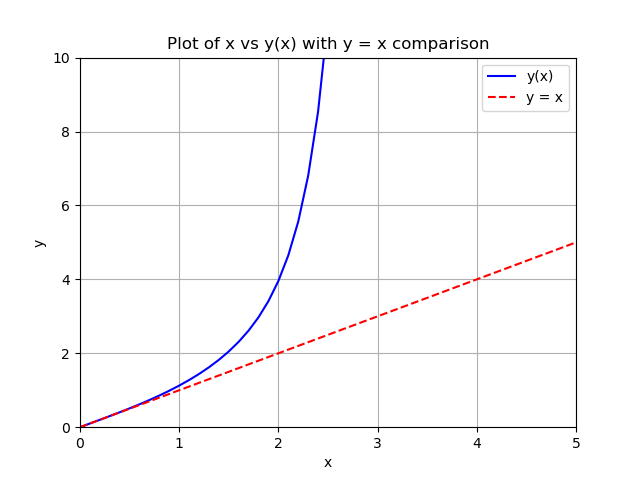
\includegraphics[width=0.5\textwidth]{figs/fig.png}
	\label{fig:Plot1}
\end{figure}

Clearly, they dont coincide hence $y=x$ is not a solution to the given differential equation.

\end{document}
